% !TeX spellcheck = it_IT
\section{Cos'è la realtà virtuale?}

La realtà virtuale (VR) è in costante evoluzione, rendendo difficile darne una definizione specifica che non decada nel giro di pochi anni. Il modo migliore per descriverla è quindi considerare gli aspetti intrinseci cruciali che prescindono la tecnologia utilizzata.La sua concezione deve essere abbastanza generale da abbracciare sia la realtà virtuale dei nostri giorni sia quella che verrà in futuro.
\subsection{Definizione della realtà virtuale}

\begin{quotation}"Indurre un comportamento premeditato attraverso l'uso di stimolazioni sensoriali artificiali in un organismo che ha una minima, se non nulla, consapevolezza dell'interferenza."\cite{VRbook}
\end{quotation}	
In questa possibile definizione di realtà virtuale compaiono quattro componenti chiave:

\begin{enumerate}
	\item \textit{Comportamento premeditato:} L'organismo sta facendo un' esperienza designata dal creatore
	che non coincide con la cognizione del mondo reale.
	\item \textit{Organismo:} Si utilizza la parola organismo poiché qualsiasi essere vivente può immergersi in un ambiente virtuale. I neurobiologi dell'Università di Monaco effettuarono i primi test sperimentali sulla VR sottoponendo dei topi da laboratorio a stimoli visivi mentre correvano su un tapis roulant sferico. Altri esperimenti sono stati fatti su scimmie, pesci, scarafaggi e moscerini.
	\item \textit{Stimolazioni sensoriali artificiali:} Attraverso degli strumenti tecnologici uno o più sensi dell'organismo vengono deviati e i loro input ordinari sono sostituiti da quelli artificiali
	\item \textit{Consapevolezza:} Durante l'esperienza virtuale l'organismo viene "ingannato" nel sentirsi presente in un mondo fittizio e non essendone conscio lo accettandolo come naturale.
\end{enumerate}

\begin{wrapfigure}{r}{0.35\textwidth} %this figure will be at the right
	\centering
	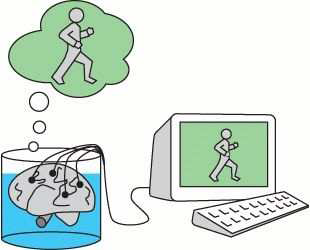
\includegraphics[width=0.25\textwidth]{figure/VRfool}
\end{wrapfigure}
Quest'ultimo fattore può sembrare frivolo, ma ci offre un'ulteriore possibilità di vedere in cosa consiste concretamente la realtà virtuale. Numerosi ricercatori di neurobiologia hanno dimostrato che il cervello di un animale sottoposto ad un'esperienza virtuale genera strutture cerebrali formate da \textit{cellule di posizione e cellule grid}, contenenti le informazioni spaziali dell'ambiente circostante, proprio come accade nella navigazione in luoghi reali.\\
Un'altra componente cruciale della realtà virtuale è l'\textit{interazione}: se la stimolazione sensoriale non dipende dalle azioni compiute dall'utente, il sistema VR viene definito \textit{open-loop} ed è il più semplice grado di virtualizzazione della realtà. In caso contrario la configurazione viene chiamata \textit{closed-loop}. In quest'ultima l'organismo ha un controllo parziale sulla manipolazione sensoriale, che potrebbe variare a seconda dei movimenti del corpo (testa,braccia,gambe,occhi,etc.), di comandi vocali, frequenza cardiaca, temperatura del corpo, resistenza elettrica cutanea (sudore). E' infatti tentante far combaciare il più possibile la simulazione con il mondo fisico, essendo ogni interazione fisica è ricreabile nel mondo virtuale ed essendo il nostro cervello più familiare con queste, accetterà più facilmente l'ambiente come naturale.

\subsection{Lo stato dell'arte}

Siamo entrati nell'età moderna della realtà virtuale grazie agli avanzamenti nelle tecnologie di visualizzazione, percezione e computazionali portate dall'industria degli smartphones. I visori di realtà virtuale ora vengono prodotti in massa e distribuiti ad un'ampia varietà di persone. Questa tendenza è molto simile alle rivoluzioni da cui nacquero i personal computer e i web browser: maggiore è il numero di persone che hanno accesso alle tecnologie, maggiori sono le possibilità di queste ultime.
\subsubsection{Applicazioni }
Al giorno d'oggi la VR è attiva nei seguenti campi \cite{VRApplications}:
\begin{enumerate}
	\item \textit{Videogiochi:}forse il campo in cui ha raggiunto la sua massima espressione ed il settore che traina la distribuzione su larga scala dei visori per la realtà virtuale.
	\item \textit{Militare:} ampiamente adottata dagli eserciti di molte nazioni per l'addestramento delle proprie truppe, poiché permette loro di imparare come reagire in situazioni ostili evitando i rischi e i costi delle vecchie simulazioni e aumentando il grado di realismo nello stress provato dai soldati. (simulatori di combattimento,medicina da campo, guida di veicoli militari,etc.)
	\item \textit{Medicina:} spesso utilizzata per la simulazione di interventi chirurgici, superamento interattivo di fobie, chirurgia robotica, diagnostica, trattamenti per persone portatrici di handicap e per l'insegnamento.
	\item \textit{Moda:} attraverso cataloghi virtualizzati e a progettazioni di negozi allestiti precedentemente in VR.
	\item \textit{Sport:} utile per migliorare le performance degli sportivi attraverso appositi ambienti virtuali, ma anche per avvicinare il pubblico mettendolo al centro dell'evento sportivo o facendogli vedere in anteprima come sarà la visuale dal suo posto dello stadio.
	\item \textit{Visualizzazione scientifica:} per mostrare più facilmente grosse moli di dati o informazioni complesse facilitando le collaborazioni interdisciplinari.
	\item \textit{Costruzione e Design:} con le esplorazioni virtuali da la possibilità di avere un feedback più realistico delle nuove strutture o soluzioni di design, come organizzazione di interni o progettazione di nuovi prodotti. prima ancora di realizzarli.
	\item \textit{Istruzione:} rende più diretto l'apprendimento in molte discipline che sarebbero difficili da visualizzare o ricordare, soprattutto nella scuola dell'infanzia.
	\item \textit{Media e informazione:} con l'utilizzo di film e documentari interattivi o di report giornalistici in cui l'utente è al centro della notizia e la può vivere in prima persona
	
\end{enumerate}

\subsubsection{Hardware e dispositivi}
Il primo passo per capire come funziona la realtà virtuale è considerare cosa costituisce un intero sistema VR.
Al contrario di quanto si possa pensare non si tratta solamente dei componenti fisici, come il visore il computer o i controllers, ma l'organismo utilizzatore è altrettanto fondamentale, che in questo capitolo verrà considerato un essere umano per facilità.\\
I sensi di una persona infatti sono centrali sia nel funzionamento della realtà virtuale che nel mondo fisico perché il cervello ne controlla la configurazione mentre riceve le informazioni da essi fornitegli formando le basi della cognizione spaziale di un individuo.\\
\begin{figure}[h]
	\centering
	\begin{minipage}[b]{0.4\textwidth}
		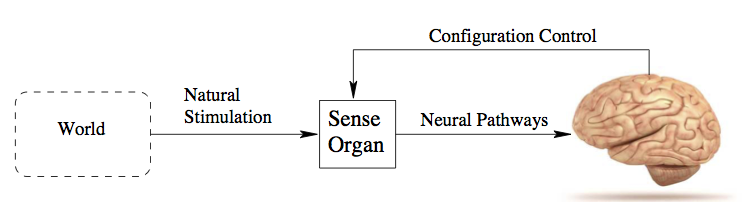
\includegraphics[width=\textwidth]{figure/RealityBB}
		{\footnotesize \centerline{(a)} \par}
	\end{minipage}
	\hfill
	\begin{minipage}[b]{0.4\textwidth}
		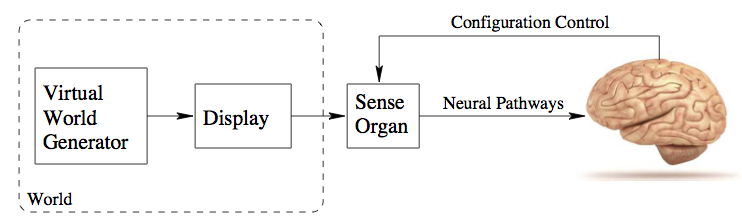
\includegraphics[width=\textwidth]{figure/VRBB}
			{\footnotesize \centerline{(b)} \par}
	\end{minipage}
	\caption{Il processo di raccolta, analisi e controllo di informazioni sensoriali nel mondo reale (a) e in quello virtuale(b).}
\end{figure}



L'hardware di una configurazione in realtà virtuale deve tenere traccia dei movimenti dell'utente per regolare gli stimoli artificiali in modo corretto, dando il desiderato senso di immersione.
Gli spostamenti della testa sono i più importanti poiché ad essa sono correlati la vista, il nostro senso predominante, e il sistema vestibolare, il quale dalle orecchie fornisce al cervello informazioni sull'equilibrio e sul moto nello spazio circostante.\cite{vestibular} Per aumentare il grado di realismo della simulazione si tende a monitorare i movimenti di braccia o gambe. Infine è in egual modo significativo prendere in considerazione l'ambiente reale circostante come parte integrante del sistema VR perché, nonostante  le stimolazioni controllate, l'utilizzatore  continuerà a percepirlo.
\begin{figure}[h]
	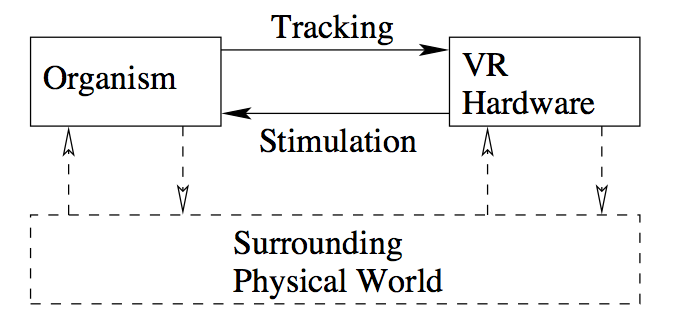
\includegraphics[width=0.45\textwidth]{figure/TrackingStimuliBB}
	\centering
	\caption{Lo schema di un sistema VR}
\end{figure}
Scendendo più nei dettagli i moderni sistemi di VR sono composti da tre componenti hardware principali: display, sensori, computer.\newline

\underline{\textit{Displays}}: \hspace{1cm} Attraverso di essi avviene la stimolazione degli organi sensoriali. Nei sistemi a \textit{CAVE} , un acronimo ricorsivo che sta per "cave automatic virtual enviroment", l'utente è avvolto da immagini 3D proiettate su sei piani di visualizzazione fissi ed immerso in un'audio sorround. Nei sistemi \textit{HMD}, head-mounted display, la configurazione consiste, come da definizione, in un visore montato sulla testa. Può essere utilizzato semplicemente lo schermo di un cell





%	Minare bitcoin
%		come si fa
%		chi lo fa.
%		guadagno
%		complessità computazionale
%		merkle hash tree
	

\section{Cos'è lo smart working?}

